\chapter{制御システム設計}
 このセクションでは,2つのセクションで提案された制御システムについて説明する. 1つは衝突検出,もう1つはブレーキシステムである.

\section{衝突検出}
 歩行者と車両の衝突を検出するために,最初にカルマンフィルターを使用して歩行者の速度を推定する.状態空間表現と推定方程式は次のように説明される.
\begin{flalign}
    \boldsymbol{x}_{\boldsymbol{h}}[k+1]=& \boldsymbol{A}_{k} \boldsymbol{x}_{\boldsymbol{h}}[k]+\boldsymbol{G}_{k} \boldsymbol{\omega}, \\
    \boldsymbol{z}_{\boldsymbol{h}}[k]=& \boldsymbol{c}_{k} \boldsymbol{x}_{\boldsymbol{h}}[k]+\boldsymbol{J}_{k} \boldsymbol{v},\\
    \hat{\boldsymbol{x}}_{\boldsymbol{h}}[k]=& \boldsymbol{A}_{k} \hat{\boldsymbol{x}}_{\boldsymbol{h}}[k-1]\nonumber \\
    &+\boldsymbol{g}[k]\left(\boldsymbol{z}_{\boldsymbol{h}}[k]-\boldsymbol{c}_{\boldsymbol{k}} \boldsymbol{A}_{k} \hat{\boldsymbol{x}}_{h}[k-1]\right)
\end{flalign}

なお

\begin{flalign}
    \boldsymbol{A}_{k}&=\left[\begin{array}{llll}{1} & {0} & {T_{s}} & {0} \\ {0} & {1} & {0} & {T_{s}} \\ {0} & {0} & {1} & {0} \\ {0} & {0} & {1} & {0} \\ {0} & {0} & {0} & {1}\end{array}\right] \nonumber\\
    \boldsymbol{G}_{k}&=\left[\begin{array}{ccccc}{\frac{1}{2} T_{s}^{2}} & {0} & {T_{s}} & {0} \\ {0} & {\frac{1}{2} T_{s}^{2}} & {0} & {T_{s}}\end{array}\right]^{T} \nonumber\\
    \boldsymbol{c}_{k}&=\left[\begin{array}{cccc}{1} & {0} & {0} & {0} \\ {0} & {1} & {0} & {0}\end{array}\right] \nonumber\\
    \boldsymbol{J}_{k}&=\boldsymbol{I}_{2} \nonumber\\
    \boldsymbol{x}_{h}[k]&=\left[\begin{array}{ll}{x_{h}[k]} & {y_{h}[k]}\end{array} \quad \dot{x}_{h}[k] \quad y_{h}[k]\right]^{T} \nonumber\\
    \boldsymbol{z}_{h}[k]&=\left[\begin{array}{cc}{x_{h}[k]} & {y_{h}[k]}\end{array}\right]^{T} \nonumber
\end{flalign}

 ここで,$\omega$,$\nu$,および$g[k]$は,それぞれシステムノイズ,観測ノイズ,および最適なカルマンゲインを示すす.$\omega$,$\nu$はホワイトノイズである. $x_h$および$y_h$は,カメラデバイスまたは道路機器によって取得される歩行者の位置.カルマンフィルターを使用すると,歩行者の速度を推定できる.
 次に,有限時間における歩行者の位置が歩行者の速度から予測される.一定期間の歩行者の速度は2次正規分布に従うと想定される.これにより,確率密度関数が一定の場合,等確率楕円が作成される.等確率楕円の方程式は次のとおり.
\begin{flalign}
    &\frac{\left(\left(x-\mu_{x}\right) \cos \alpha+\left(y-\mu_{y}\right) \sin \alpha\right)^{2}}{\left(c \sigma_{u}\right)^{2}}\nonumber\\
    &+\frac{\left(-\left(x-\mu_{x}\right) \cos \alpha+\left(y-\mu_{y}\right) \sin \alpha\right)^{2}}{\left(c \sigma_{v}\right)^{2}} =1
\end{flalign}

なお

\begin{flalign}
    \sigma_{u}^{2} &=\frac{\sigma_{x}^{2}+\sigma_{y}^{2}+\sqrt{\left(\sigma_{x}^{2}-\sigma_{y}^{2}\right)+4 \sigma_{x y}^{2}}}{2} \nonumber\\
    \sigma_{v}^{2} &=\frac{\sigma_{x}^{2}+\sigma_{y}^{2}-\sqrt{\left(\sigma_{x}^{2}-\sigma_{y}^{2}\right)+4 \sigma_{x y}^{2}}}{2} \nonumber\\
    \alpha &=\arctan \frac{\sigma_{u}^{2}-\sigma_{x}^{2}}{\sigma_{x y}} \nonumber
\end{flalign}

 ここで,$\mu_x$と$\mu_y$は平均値,$\sigma_x$,$\sigma_y$は標準偏差,$\sigma_{xy}$は歩行者の速度の共分散である.さらに,$\alpha$は等確率楕円の角度を示す. $c$は確率密度関数$f$に依存し,$c$と$f$の関係を表1に示す.
\begin{table}[]
    \centering
    \caption{$f$と$c$の関係}
    \begin{tabular}{|l|l|}
    \hline
    f     & c      \\ \hline
    0.393 & 1.000  \\ \hline
    0.500 & 1.177  \\ \hline
    0.900 & 2.146 \\ \hline
    0.950 & 2.448 \\ \hline
    0.990 & 3.035  \\ \hline
\end{tabular}
\end{table}
したがって,式(13)は1秒での歩行者の予測位置を示す.一方,入力なしの車両の予測位置は次のように定式化される.
\begin{flalign}
    \hat{\boldsymbol{x}}[k+i | k]=\boldsymbol{A}^{i} \hat{\boldsymbol{x}}[k | k]+\boldsymbol{B} F_{r}
\end{flalign}

 $i = 1, 2, ..., Hp$および$H_p$は予測周期である.次に,衝突検出について説明する.車両と歩行者が衝突する可能性があるかどうかは,以下の式を計算することで確認できる.
\begin{flalign}
D&=\frac{(a+b)^{2}}{\left(c \sigma_{u}\left(i T_{s}+\tau\right)+R_{h}\right)^{2}}+\frac{(-a+b)^{2}}{\left(c \sigma_{v}\left(i T_{s}+\tau\right)+R_{h}\right)^{2}}\\
a&=\left(\hat{s}_{1}[k+i | k]-\mu_{x}\left(i T_{s}+\tau\right)-x_{h}\right) \cos \alpha \nonumber\\
b&=\left(\hat{x}_{2}[k+i | k]-\mu_{y}\left(i T_{s}+\tau\right)-y_{h}\right) \sin \alpha \nonumber
\end{flalign}
 $R_h$と$\tau$は,それぞれ歩行者の安全ゾーンの半径と計算のむだ時間を示す. $x_h$と$y_h$は歩行者の現在位置,$\mu_x$と$\mu_y$は一定期間内の歩行者の速度の平均. Dが1未満の場合,車両は歩行者の予測位置にあるため,衝突を避けるために減速する必要がある.車両停止位置の指令値は,次のように$x$と$y$の連立方程式を解くことによって決定される.
\begin{equation}
    \left\{\begin{array}{c}{\dfrac{\left(a^{\prime}+b^{\prime}\right)^{2}}{\left(c \sigma_{u}\left(i T_{s}+\tau\right)+R_{h}\right)^{2}}+\dfrac{\left(-a^{\prime}+b^{\prime}\right)^{2}}{\left(c \sigma_{v}\left(i_{c} T_{s}+\tau\right)+R_{h}\right)^{2}}=1} \\
    {y=\boldsymbol{x}_{3}[k | k] \tan \theta x-\boldsymbol{x}_{1}[k | k] \boldsymbol{x}_{3}[k | k] \tan \theta+\boldsymbol{x}_{2}[k | k]}\end{array}\right.\\
\end{equation}

\begin{flalign}
    a^{\prime}&=\left(x-\mu_{x}\left(i_{c} T_{s}+\tau\right)-x_{h}\right) \cos \alpha \nonumber \\
    b^{\prime}&=\left(y-\mu_{y}\left(i_{c} T_{s}+\tau\right)-y_{h}\right) \sin \alpha \nonumber
\end{flalign}

 $i_c$は,式(15)の$D\leq1$を満たす最小の$i$である.車両の現在位置により近い解が衝突回避の制限停止位置として採用され,$i_cT_s$の停止司令点は制限位置から一定の距離にある位置となる.図3に,衝突検出のプロセスの概要を示す.

\begin{figure}[]
    \centering
    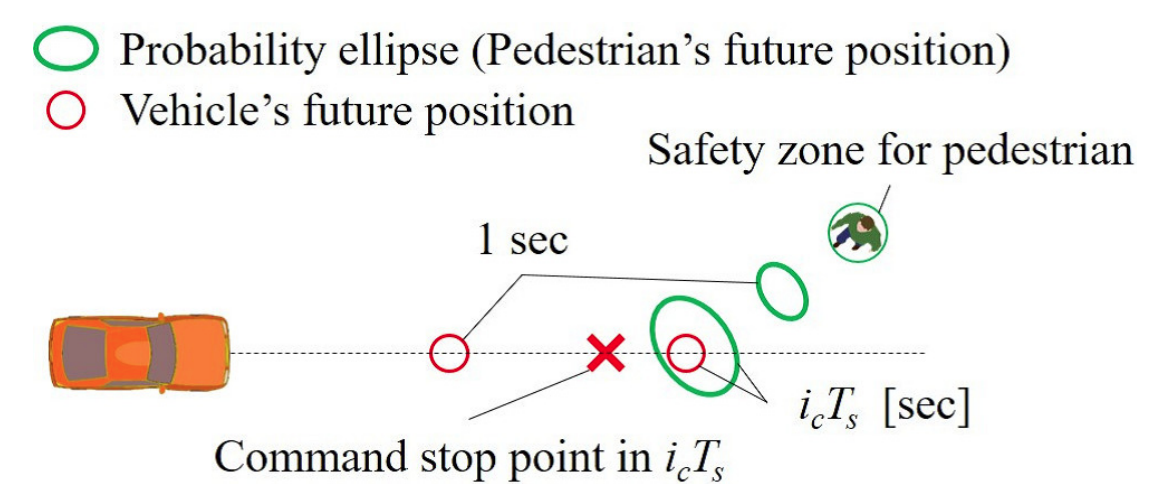
\includegraphics[width=8cm]{./fig/fig3.png}
    \caption{衝突検知の概要}
\end{figure}


\section{ブレーキコントロールシステム}
 モデル予測制御(MPC)は,車両を減速して$i_cT_s$の停止位置で停止するために使用される. MPCは,入力を最適化すると同時に,いくつかの制約を使用して各時点で将来の応答を予測する制御方法である.評価関数は次のとおり.
\begin{flalign}
    V[k]=\|\boldsymbol{Z}[k]-\boldsymbol{T}[k]\|_{Q}^{2}+\|\Delta \boldsymbol{U}[k]\|_{R}^{2}
\end{flalign}

なお

\begin{flalign}
    \mathbf{Z}[k]&=\left[\begin{array}{c}{z\left[k+H_{w} | k\right]} \\ {\vdots} \\ {\vdots} \\ {z\left[k+H_{p} | k\right]}\end{array}\right] \nonumber\\
    \boldsymbol{T}[k]&=\left[\begin{array}{c}{r\left[k+H_{w} | k\right]} \\ {\vdots} \\ {r\left[k+H_{p} | k\right]}\end{array}\right] \nonumber\\
    \boldsymbol{\Delta U}(k)&=\left[\begin{array}{c}{\Delta \hat{u}(k | k)} \\ {\vdots} \\ {\Delta \hat{u}\left(k+H_{u}-1 | k\right)}\end{array}\right] \nonumber
\end{flalign}

 $u$は制御範囲. QおよびRの説明は次のとおり.

\begin{flalign}
    \boldsymbol{Q}&=\left(\begin{array}{cccc}{\boldsymbol{Q}\left(H_{w}\right)} & {0} & {\cdots} & {0} \\ {0} & {\boldsymbol{Q}\left(H_{w}+1\right)} & {\cdots} & {0} \\ {\vdots} & {\vdots} & {\ddots} & {\vdots} \\ {0} & {0} & {\cdots} & {Q\left(H_{p}\right)}\end{array}\right) \nonumber\\
    \boldsymbol{R}&=\left(\begin{array}{cccc}{\boldsymbol{R}(0)} & {0} & {\cdots} & {0} \\ {0} & {\boldsymbol{R}(1)} & {\cdots} & {0} \\ {\vdots} & {\vdots} & {\ddots} & {\vdots} \\ {0} & {0} & {\cdots} & {\boldsymbol{R}\left(H_{u}-1\right)}\end{array}\right) \nonumber
\end{flalign}

 ここで,$H_w$は入力デッドタイムを示すウィンドウパラメーターである. $Q$と$R$は,それぞれ出力誤差と入力変化の重み行列である.式(17)の右側の第一項は司令値からの誤差を減らす効果があり,2番目の項は入力の突然の変化を抑制する. $r[k + i]$は次のように決定される.
\begin{flalign}
    \boldsymbol{r}[k+i]^{T}=\left(\begin{array}{lll}{x_{s}} & {y_{s}} & {0}\end{array}\right) \quad i_{c} \leq i \leq H_{p}
\end{flalign}


 式(18)は,$i_cT_s$ [sec]以降の車両位置を示す.ちなみに,出力と入力の変更と入力の制約は次のとおり.
\begin{flalign}
    \left|\hat{z}_{1}[k+i | k]-z_{1}[k | k]\right| \leq\left|x_{s}-z_{1}[k | k]\right| \\
    \left|\hat{z}_{2}[k+i | k]-z_{2}[k | k]\right| \leq\left|y_{s}-z_{2}[k | k]\right| \\
    |\Delta \hat{u}[k+i | k]| \leq \Delta u_{m a x} \\
    -\hat{\mu}_{\max } M g \leq u[k+i | k] \leq 0
\end{flalign}

 式(19)〜(20)は,コマンドの停止点を超えて実行されないための役割. (21)は,入力の変化がチューニングパラメーターである$\Delta u_{max}$より小さいことを示している. 式(22)は,タイヤの力を摩擦円理論で決定される最大制動力よりも小さくする. 式(19)〜(22)に示す制約の下,最適な入力変化$\Delta u[k | k]$が計算される. したがって,各車輪の最適な制動力は次のように決定される.
\begin{flalign}
    F_{d}^{c m d}=u[k-1]+\Delta u[k | k]
\end{flalign}

 MPCは,モデリングエラーを補正するためにフィードバックループが必要な開ループコントローラーである. したがって,MPCの内部でタイヤ力のフィードバックループを提供することが提案する. したがって,ブレーキ装置によって生成される基準トルクは次のように決定される.
\begin{flalign}
    T_{m}^{r e f}=\frac{K_{i}}{s}\left(F_{d}^{c m d}-\hat{F}_{d}\right)
\end{flalign}

 ここで,$K_i$および$\hat{F}_{d}$はそれぞれ,積分ゲイン,および駆動力オブザーバー(DFOB)によるタイヤ力の推定値を示す.

\section{オブザーバー設計}
 このセクションでは,タイヤの力と走行抵抗を推定する方法について説明する. タイヤの力を推定するために,駆動力オブザーバー(DFOB)が使用される. DFOBは,外乱トルクを正確に推定できる外乱オブザーバー(DOB)に基づいている. DFOBは次のように定式化される.
\begin{flalign}
    \hat{F}_{d}=\frac{1}{r_{w}}\left(\frac{g_{c u t}}{s+g_{c u t}}\left(T_{m}^{r e f}+g_{c u J} J \omega\right)-g_{c u t} J \omega\right)
\end{flalign}

 ここで,$g_{cut}$はローパスフィルター(LPF)のカットオフ周波数を示す. DFOBのブロック図を図4に示す. 制御性能を向上させるには,駆動抵抗$F_r$を推定する必要があり,式(26)を使用して推定できる. 走行抵抗推定器のブロック図を図5に示す.
\begin{flalign}
    \hat{F}_{r}=M \frac{g_{c u t}}{s+g_{c u t}} a-n \hat{F}_{d}
\end{flalign}

\begin{figure}[]
    \centering
    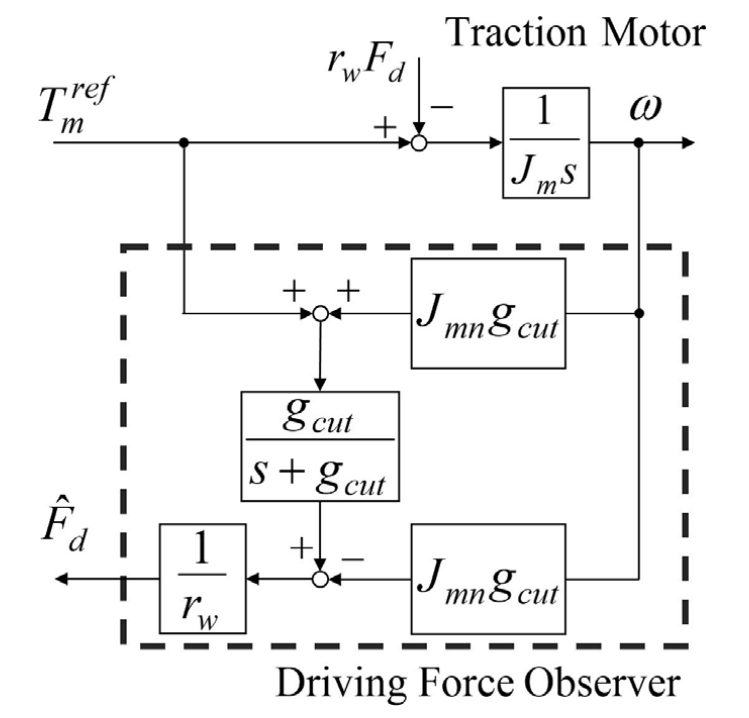
\includegraphics[width=8cm]{./fig/fig4.png}
    \caption{DFOBのブロック図}
\end{figure}
\begin{figure}[]
    \centering
    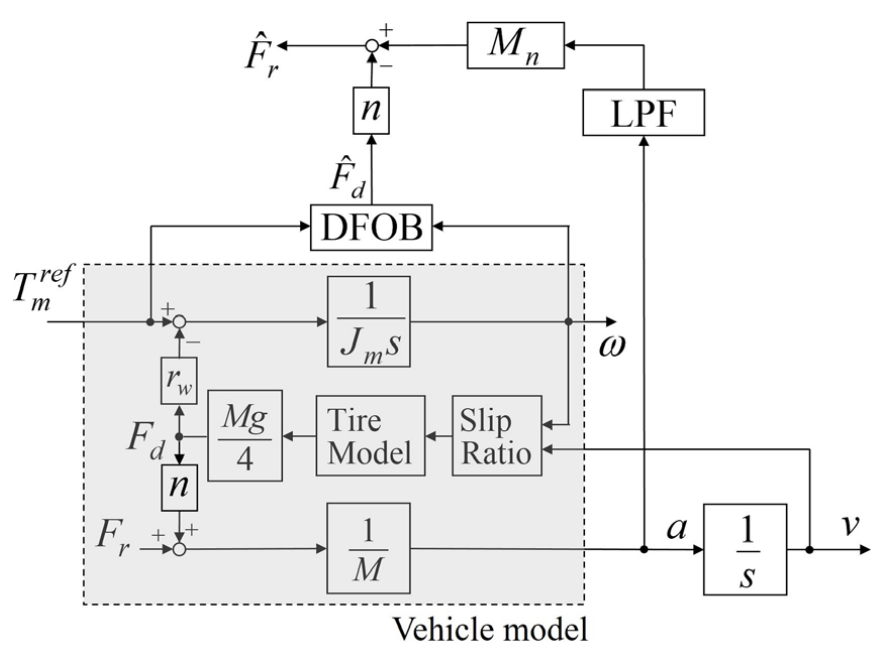
\includegraphics[width=8cm]{./fig/fig5.png}
    \caption{走行抵抗推定のブロック図}
\end{figure}

 aは車両の縦加速度. $\mu$は式(7)で推定でき,$\lambda$は式(8)で計算される. $lambda$と$\mu$を連続して取得して,最大摩擦係数$μ_{max}$は,最小二乗法(LSM)を使用して$\mu-\lambda$曲線を2次関数に近似することによって推定され,式のMPCの制約として$\mu_{max}$を設定する.
 最後に,ブレーキシステム全体を図6に示す.
\begin{figure}[]
    \centering
    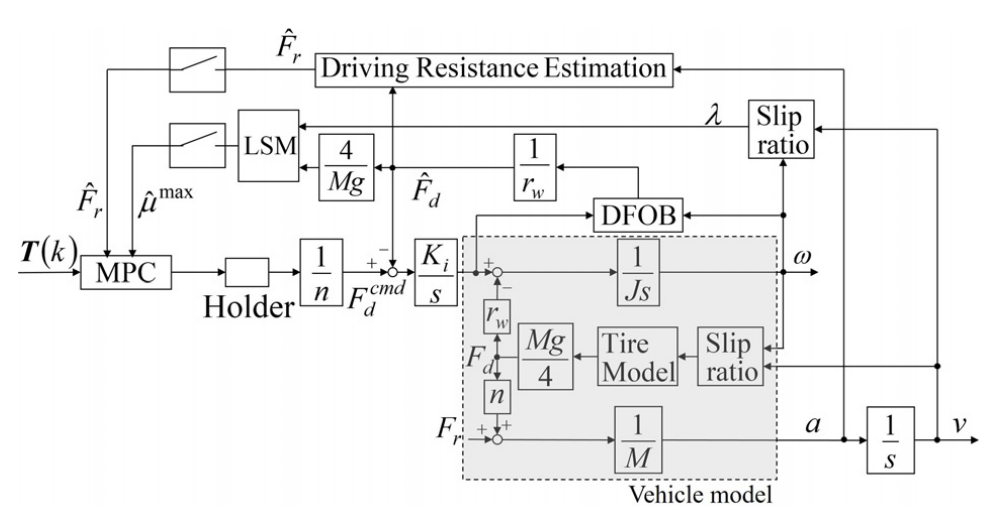
\includegraphics[width=8cm]{./fig/fig6.png}
    \caption{ブレーキシステム全体のブロック図}
\end{figure}
